\chapter{Project Plan}
\label{ch:project_plan}
In the following section, the project plan of the proposed master's thesis is discussed.
The project plan consists of a work plan, time schedule, and risk assessment.
The work plan defines the project objectives, milestones, tasks, and deliverables and is presented in \autoref{sec:work_plan}.
The time schedule represents the mapping of the proposed work plan to calendar weeks and is discussed in \autoref{sec:time_schedule}.
The risk assessment evaluates technical and non-technical risks for the proposed project plan and is discussed in \autoref{sec:risk_assessment}.

\section{Work Plan}
\label{sec:work_plan}
The work plan structures the proposed thesis into\dots 
\todo{Workplan, Incremental Parts ("inkremente"), Dependencies, Deliverable-Duration-Limitation, time schedule (milestones, temporal dependencies)}

\section{Time Schedule}
\label{sec:time_schedule}
\dots
\begin{figure}
    \centering
    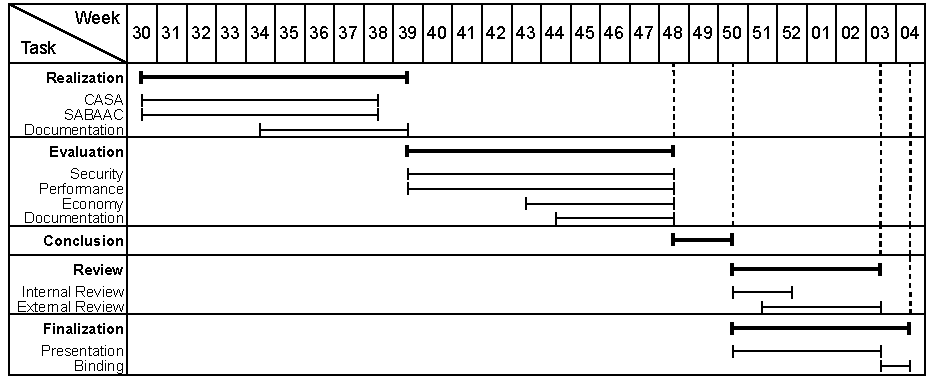
\includegraphics[width=1.0\linewidth]{figures/timeplan.drawio.pdf}
    \caption{Time schedule of the proposed master's thesis.}
    \label{fig:timeplan}
\end{figure}

\section{Risk Assessment}
\label{sec:risk_assessment}
The risk assessment identifies technical as well as project management risks and assesses their impact on the proposed project plan.\dots
\todo{Find, analyse, describe, estimate risks}
\todo{Provide mitigation ideas for each risk}
